\section{Motivation}

Personal, academic, and industrial motivations drive this thesis. 

This research is conducted in collaboration with \textit{Epidemic Sound AB (ES)} \cite{EpidemicSite}, a prominent Swedish company that provides a global library of over 40,000+ royalty-free soundtrack music and 90,000+ sound effects, and the \textit{Music Technology Group (MTG)} at Universitat Pompeu Fabra in Barcelona, Spain. 

The MTG specializes in developing new technologies related to sound and music, including music information retrieval, digital signal processing, computational models of music perception and cognition, and interactive music systems. 

The collaboration with Epidemic Sound and the MTG aims to deepen our understanding of music and its fundamental structures, potentially leading to advancements and benefits for the company's technical products, services, and MIR academic research.

\subsubsection{Personal motivation}

As a music enthusiast, professional musician, and scholar, I am passionately committed to exploring the foundational elements of musical composition, investigating the diverse techniques employed in creating musical works, and deciphering the intricate relationships among them. This passion fuels my quest for knowledge on extracting valuable information embedded within music in any domain, being my main interest in the audio and symbolic domain, contributing to developing more sophisticated and effective music-related technologies and solutions in the industrial landscape.

I advocate for exposure as the primary method of learning music, emphasizing the importance of immersing oneself in various musical experiences to foster a holistic understanding of music as an art form. Individuals can cultivate well-rounded musical expertise by engaging with different styles, genres, techniques, and learning approaches, ultimately promoting creativity and experimentation.

On top of that, I argue that MIR research needs to incorporate a more balanced approach that considers the interdisciplinary nature of music and the importance of other domains beyond DSP.

\subsubsection{Academic motivation}

The emergence of self-supervised models that learn embedding spaces for retrieving musical content from audio signals has unveiled new opportunities in academic research. By capturing high-level semantic information from raw audio data in an unsupervised manner, these models can potentially revolutionize various aspects of the music industry. Their applications encompass music information retrieval, sharing learned latent representations for MIR \cite{HamelTransferSimilarity}, and fostering interdisciplinary research and innovation in musicology, computer science, and artificial intelligence.

\subsubsection{Industrial and corporate motivation}

In the industrial and corporate realm, the embedding spaces generated by these models can be utilized to create personalized and intelligent music recommendation systems \cite{Chen2020LearningRecommendation}\cite{epidemic}, facilitate effective enforcement of intellectual property rights, and contribute to the development of more sophisticated audio editing-production tools and technical products \cite{WonEmotionStories}. These advancements ultimately enhance our interaction with music in the digital age, promoting innovation and collaboration across the music industry.

While it is true that the theoretical foundations of machine learning can be traced back to the pioneering work of figures such as Alan Turing and Claude Shannon in the mid-twentieth century, we are currently experiencing a period of significant breakthroughs in AI research \cite{Vaswani2017AttentionNeed}. These breakthroughs have facilitated the implementation of AI in widely used products \cite{OpenAI2023GPT-4Report}. Many researchers and corporations are keen to stay abreast of these developments and contribute to this exciting and rapidly evolving field.

\subsection{About music aural skills and high-level perceptual concepts}

I have consistently been inspired by musicians and researchers who strive to uncover musical ground truth within an existing tonal paradigm, such as Heinrich Schenker and his school of thought \cite{Komar1959SchenkersStructure}, particularly by challenging it, exemplified by Arnold Schoenberg \cite{Samson1974SchoenbergsMusic}, George Russell \cite{LydianRussell} or Ernst Levy \cite{LevyAHarmony}. These approaches aim to identify abstract concepts that reinforce or disrupt the tonal foundation. Their ultimate goal is to advance the tonal landscape, providing musicians with a dependable playground for growth, development, and further understanding tonal and atonal paradigms.

%%%%%%%%%%%%%%%%%%

\begin{figure}[ht]
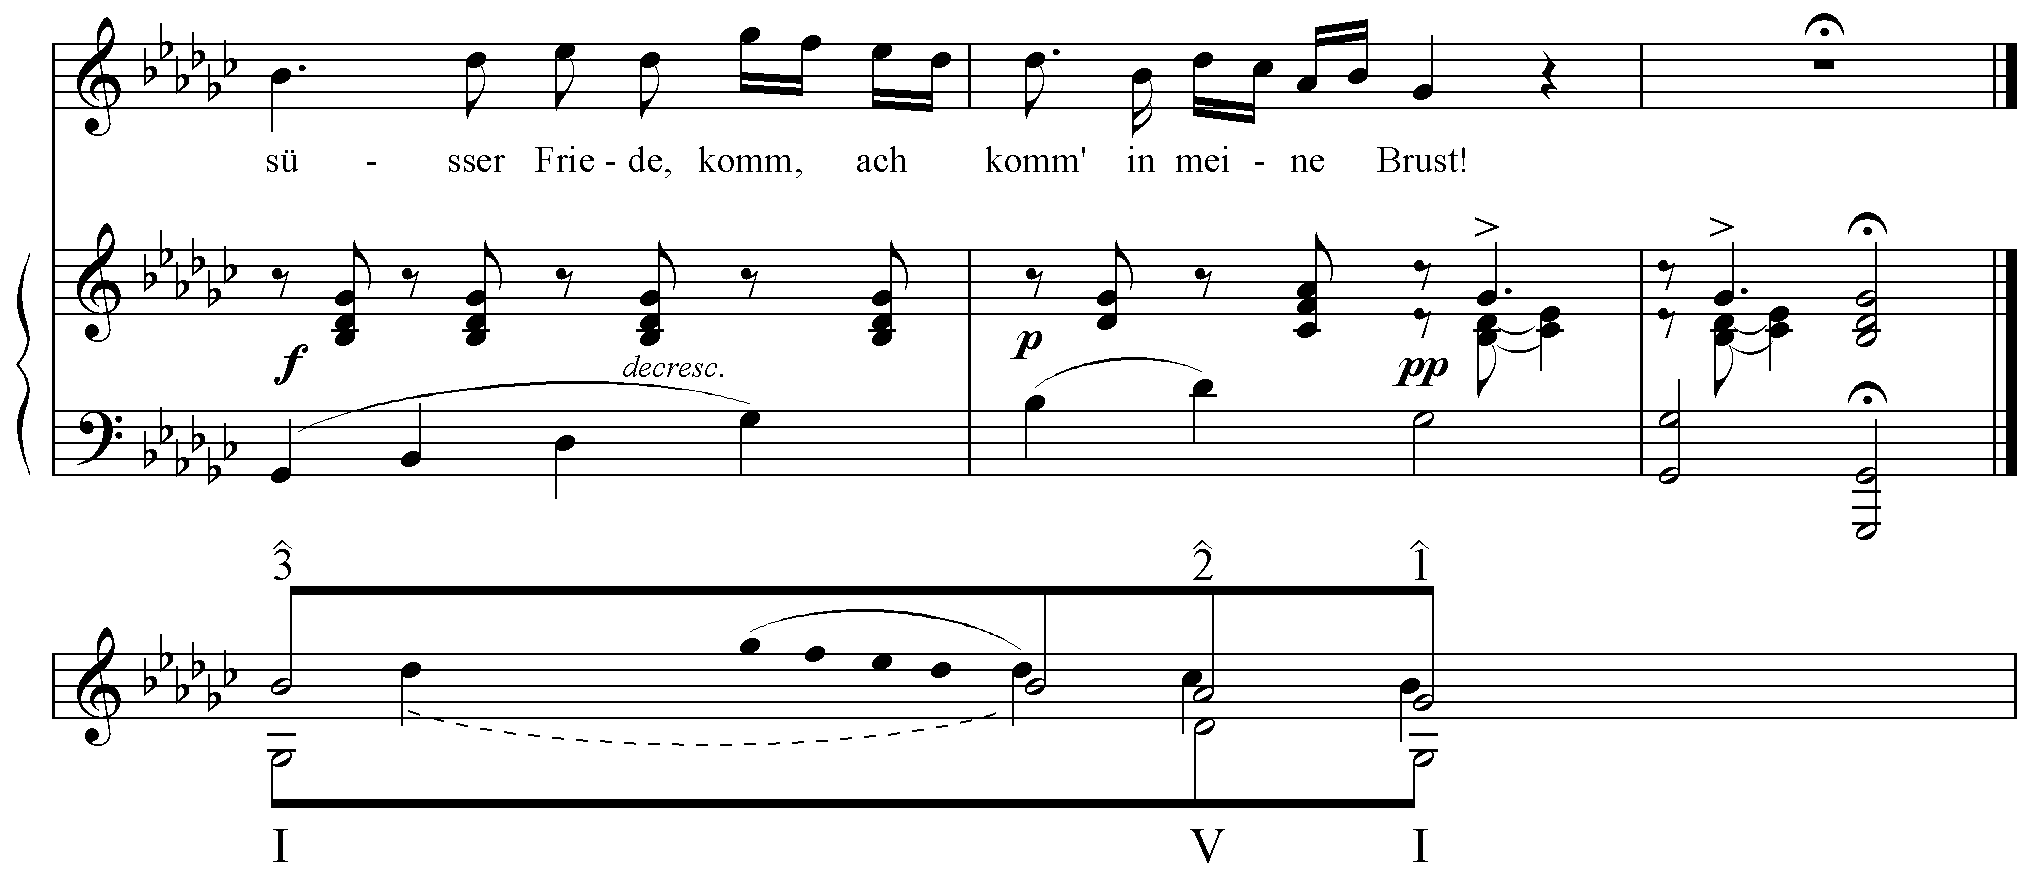
\includegraphics[clip,width=\columnwidth]{figures/schenkerian analysis/SchubertOp4no3.png}% 
\caption[Excerpt of \textit{Wandrers Nachtlied, Op. 4, D. 224} by Franz Schubert.]{\small{Small excerpt of \textit{Wandrers Nachtlied, Op. 4, D. 224} by Franz Schubert. Passage's original score, the schenkerian unfolding of the melody, the chord degrees analysis, and their tonal function.}}
\label{fig:Wandrers Nachtlied, Op. 4, D. 224}
\end{figure}